%%%%%%%%%%%%%%%%%%%%%%%%%%%%%%%%%%%%%%%%%%%%%%%%%%%%%%%%%%%%%%%%%%%%%%%%
% RevTeX 4.1 LaTeX
% Kevin C. Young
% Scalable & Secure Systems Research (08961)
% Thu Mar  5 15:29:19 PST 2015
%%%%%%%%%%%%%%%%%%%%%%%%%%%%%%%%%%%%%%%%%%%%%%%%%%%%%%%%%%%%%%%%%%%%%%%%

\documentclass[aps,nofootinbib,pra,notitlepage,twocolumn]{revtex4-1}

\usepackage{amsfonts,amsmath,amssymb,amsthm}
\usepackage{array,bm,color}
\usepackage{epsfig,graphicx,nomencl,revsymb4-1,upgreek,url}
\usepackage{hyperref}
\usepackage{algorithm}
\usepackage{algpseudocode}
\usepackage{graphicx}
% \usepackage[justification=justified,font=small]{caption}
\graphicspath{{./figures/}}
\hypersetup{colorlinks=true, pdfauthor=Kevin C. Young, pdftitle=Decorrelating Errors}
\newcommand{\tr}{{\rm Tr\thinspace}}
\newcommand{\bra}[1]{\ensuremath{\left\langle{#1}\right\vert}}
\newcommand{\ket}[1]{\ensuremath{\left\vert{#1}\right\rangle}}
\newcommand{\braket}[2]{\left\langle #1 | #2 \right\rangle}
\newcommand{\ketbra}[2]{\left| #1 \right\rangle\!\!\!\,\left\langle #2 \right|}
\newcommand{\abs}[1]{\left\vert #1 \right\vert}
\newcommand{\expect}[1]{\ensuremath{\left\langle{#1}\right\rangle}}
\newcommand{\timeorder}{\ensuremath{\underset{\leftarrow}{\mathcal{T}}}}
\newcommand{\ident}{{\mathbb1}}
\newcommand{\order}[1]{\mathcal{O}\left( #1 \right)}
\newcommand{\diag}[1]{\mathrm{diag}\{#1\}}
\newcommand{\trans}[1]{#1^\mathsf{T}}
\newcommand{\T}{\mathsf{T}}

\newcommand{\erf}[1]{Eq.~(\ref{#1})}
\newcommand{\needcite}{{\color{blue}\textsuperscript{[citation needed]}}}
\newcommand{\note}[1]{{\color{red}[#1]}}
\newcommand{\kcy}[1]{{\color{red}[#1]{\rm{KCY}}}}

%-------------Header begins here----------------------------------------
\begin{document}
% \tableofcontents
\title{Decorrelating Errors in Quantum Gates by Random Gate Synthesis}

\author{Anthony Polloreno}
\email[Email: ]{anthony@rigetti.com}
\affiliation{Rigetti Computing, Berkeley, CA}

\author{Kevin C. Young}
% \email[Corresponding author: ]{kyoung@sandia.gov}
\affiliation{Sandia National Laboratories, Livermore, CA}

\date{\today}

\begin{abstract}
Thresholds for fault-tolerant quantum computation are often calculated assuming a noise model in which errors are uncorrelated. While convenient for simulation, these error models are often unphysical. Work by Preskill and others has shown that arbitrarily long computations may be performed even in the presence of spatial correlation, provided the correlation is sufficiently weak and decays sufficiently quickly with distance, but at the cost of a significantly lower threshold. The success of algebraic decorrelation methods, such as dynamical decoupling, demonstrate that quantum control techniques are capable of reducing temporal noise correlations. We propose to introduce similar methods to effect the spatial decorrelation of errors in quantum circuits, thereby increasing the threshold for fault-tolerant computation in such systems.
\end{abstract}

\pacs{}

\maketitle

\section{Introduction}

Steady progress has been made in the theory of quantum error correction, proving higher thresholds for increasingly general models of noise \cite{Aharonov2006} \kcy{more recent citations}. These results show that quantum computation is feasible in principle, however recent NISQ \cite{Preskill2018} devices have noise that is not only often above thresholds, but that also violates fundamental assumptions made by the models used in these results, such as Markovianity \cite{Kitaev1997} and independence of errors\needcite. With these assumptions violated, promises about system performance and correctness are difficult to make.

There are many ways in which device noise can fail to be Markovian,\cite{Kelly2018, BlumeKohout2017}, and even when the noise \textit{is} Markovian, many models make simplifying assumptions about the structure of the noise. For instance, Pauli channels are often used to model systems\needcite due to their classical simulability\needcite, despite their unrealistic form. Some authors have then taken the approach of using these easily-understood models to upper bound the error in a real system by \textit{honestly} representing them \cite{Puzzuoli2014}. This approach is correct and rigorous, but produces overly-pessimistic bounds on device performance.

Other authors have addressed these problems \cite{Wallman2016, Campbell2017, Heim2016} by using circuit compilation to remove correlated noise. Given a process that is generated by a sequence of channels with some unknown and potentially channel dependent error, coherent errors can be averaged away into incoherent error. Indeed, some of these routines have been demonstrated experimentally \cite{Ware2018}, and been shown to reduce the coherence of noise. However, this benefit comes at the cost of additional compilation steps, which may in general increase circuit depth and require more sophisticated classical preprocessing.

\begin{figure}
  \centering
  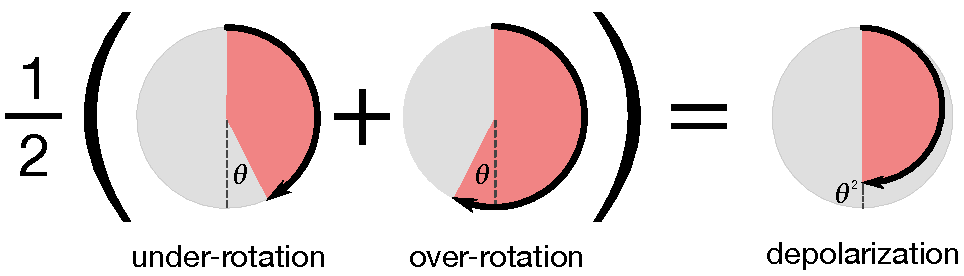
\includegraphics[width=\columnwidth]{simple_example.pdf}
  \caption{An example of a balanced control solution. Using optimal control, two implementations of a $Z_\pi$ gate are designed to have equal and opposite sensitivity to errors (if one implementation over-rotates by angle $\theta$, then the other \emph{under}-rotates by $\theta$). Each time the gate is used, one of these implementations is chosen at random. The resulting quantum channel is equivalent to a perfect implementation of the gate followed by dephasing of $\order{\theta^2}$.}
  \label{fig:simple_example}
\end{figure}

In this Letter, we take a different approach to address these problems at the gate synthesis level. We propose to inject additional decorrelating randomness into the system through the use of \emph{balanced control solutions} (BCSs). BCSs are families of control solutions that approximate the same target gate, but with balanced errors for any given instance of the noise Hamiltonian. That is, for a target gate, $U_T$, we seek a family of control solutions, $c_i(t)$, each implementing an approximation $U_i$ to the target gate, such that the family of unitary approximations is \emph{balanced}. A balanced family is one which satisfies, for some small $\alpha$,
\begin{equation}\label{eq:1}
  \frac{1}{N}\sum_{i=1}^N \omega_i U_i \rho U_i^\dagger = DPN[\alpha]\left(U_T \rho U_T^\dagger \right)
\end{equation}

Where $DPN[\alpha](\rho)$ is a \textit{generalized} depolarizing noise channel with strength $\alpha$. (For the rest of this paper, we will refer to them as just depolarizing channels.) Such a channel is defined as:
\begin{equation}\label{eq:2}
  DPN[\alpha](\rho) \rightarrow (1-\alpha)\rho + \alpha\sum p_i \sigma_i\rho\sigma_i
\end{equation}
with $p_i$ summing to one. This means that on average, the unitary approximations implement the target unitary followed by a small depolarizing channel. The task of constructing the BCSs will fall to optimal control.

This techique can be used to turn coherent error into incoherent errorr, correlated error into uncorrelated error, and therefore non-Markovian noise into more Markovian noise. This is particularly, since many routines exist that can assess the quality of a gateset, however in the presence of non-Markovianity most of them become unreliable.

For example, randomized benchmarking and tomography will report incorrect answers without any syndrome \cite{Merkel2013}, and gateset tomography will report that the gateset failed to be Markovian, but will fail to diagnose in what way it was non-Markovian. Because BCSs can make error channels look more depolarizing, the correlations in the noise can be reduced, and the process can be made much closer to Markovian. In addition, we will show that this comes at no real cost to the fidelity of the implemented gate. Finally, unlike in \cite{Wallman2016, Campbell2017, Ware2018} this method of coherent error mitigation is cheap to implement - it only requires a random choice of pulse definition at run time, in addition to the extra storage required to store the pulse shapes - no classical preprocessing or runtime frame tracking is required.


\section{A Simple Example}
As a somewhat trivial example, consider a single-qubit rotation-angle error, such as result from stochastic laser amplitude fluctuations. A BCS may consist of an $X_\pi$ pulse, as well as an $\bar X_\pi$ pulse (i.e., a clockwise and counter clockwise rotation of the qubit). In the case of excess amplitude, the $X_\pi$ pulse will result in an over-rotation error, while the $\bar X_\pi$ pulse results in an \emph{under}-rotation error. When it comes time to perform the target gate in a quantum circuit, one member of the BCS is chosen uniformly at random. This has the effect of decreasing the norm of the noise channel and decorrelating the over-rotation error (Figure \ref{fig:simple_example}). In this simple example, we can solve the minimization problem given by equation \ref{eq:minimization} analytically. In particular, if we choose the weights in \ref{eq:1} such that $\omega_i=1$, and we choose to represent our gates in the vectorized superoperator representation, then:

\begin{equation}
  \begin{gathered}
    \frac{1}{2}(X^*_{\pi + \epsilon}\otimes X_{\pi + \epsilon} + \bar X^*_{\pi + \epsilon}\otimes \bar X_{\pi + \epsilon}) \\
    = (\sin^2{\frac{\pi + \epsilon}{2}}I\otimes I + \cos^2{\frac{\pi + \epsilon}{2}}X\otimes X)X\otimes X \\
    \approx ((1 - \epsilon^2)I\otimes I + \epsilon^2X\otimes X)X\otimes X
  \end{gathered}
\end{equation}

Therefore, for a rotational error of angle $\epsilon > 0$, we see that $X_\pi$ and  $\bar X_\pi$  form a BCS, with $\alpha\approx\epsilon^2$.



\section{Optimal Control Problems}\label{ocp}
\subsection{Random Gate Synthesis}
Generating BCSs can be done in a variety of ways, using any quantum optimal control technique \cite{Caneva2011, Machnes2018} to find a family of controls. For simplicity in this paper we use the GRAPE algorithm to generate candidate pulseshapes to approximate the target gate. First described in \cite{Khaneja2005}, the GRAPE (GRadient Ascent Pulse Engineering) algorithm is a technique for finding piecewise constant control sequences that approximate a desired unitary, $U_T$. Defining our uncontrolled Hamiltonian as $H_0$, our control Hamiltonians as $H_{i\neq 0}$, and our \textit{control matrix} $u_{ij}$ as containing control amplitude associated with the $i^{th}$ time step and the $j^{th}$ hamiltonian, we can write our approximate unitary at any timestep as
\begin{equation}\label{eq:3}
  U_i = \exp\{-i\Delta t(H_0 + \sum_{j=1}^{n}u_{ij}H_{j}\}
\end{equation}
Then, to measure the simularity of our approxiate unitary $U_n$ to our target unitary $U_T$, we can define a cost function $J(U) = Tr\{U_T^{\dagger}U_n\}$.

To optimize this cost function we can perform the following standard update loop for some threshold value $\varepsilon > 0$ and step size $\delta > 0$:
\begin{algorithm}[H]
\floatname{algorithm}
  \caption{\textsc{\textbf{Gradient Ascent}}}
  \begin{algorithmic}
    \While{$J(U_n) < (1-\varepsilon$)}
    \State $u_{ij} \rightarrow u_{ij} + \delta\frac{\partial J(U)}{\partial u_{ij}}$
    \For{$1 \leq i \leq n$}
    \State $U_i \rightarrow \exp\{-i\Delta t(H_0 + \sum_{i=0}^{n}u_{ij}H_j)\}$
    \EndFor
    \State $U \rightarrow \prod_{i=1}^nU_i$
    \EndWhile
  \end{algorithmic}
\end{algorithm}

In general these gradients can be computed by propagating partial derivatives of the cost function with respect to control parameters through each timestep of the  via the chain rule. However, in \cite{Khaneja2005} Khaneja et al. derive a simple update formula that is correct to first order. In particular one can show that:
\begin{equation}\label{eq:update}
  \begin{split}
\frac{\partial J(U)}{\partial u_{ij}} = -2Re\{\braket{{U_{j+1}^{\dagger}...U_N^{\dagger} U_T}}{i\Delta tH_jU_j...U_1}\\
\braket{U_j...U_1}{U_{j+1}^{\dagger}...U_N^{\dagger} U_T}\} +  \mathcal{O}(\Delta t^2)
  \end{split}
\end{equation}


In our numerical results in Section \ref{1Q Gates} and \ref{2Q Gates}, we have modified the update step in \ref{eq:update} to instead use approximately the following gradient:
\begin{align}\label{quadrature}
\int p(\vec{\delta})\frac{\partial J(U(\vec{\delta}))}{\partial u_{ij}} d\vec{\delta}
\end{align}
with $p(\vec{\delta})$ Gaussian distributed. This technique has been used in previous works such as \cite{Goerz2014} to ensure that the optimal control results are robust over a wide range of errors, and we approximate this integral in this paper by using Gaussian quadrature.\needcite Doing this ensures that the family of controls produced by our routine, $U_i$, perform moderately well over a range of control errors that might occur.

Concretely we consider a Hamiltonian of the following form:
\begin{equation}\label{eq:2}
  H(t) = \delta_0H_0 + \sum_{i=1}^n (1 + \delta_i)c_i(t)H_i
\end{equation}
for control Hamiltonians $H_i$, free evolution Hamiltonian $H_0$ and random variables $\delta_i$, that model some small uncertainty in parameters in the Hamiltonian. Such a model might describe a superconducting qubit quantum processor where control amplitudes for the RF pulses vary over time, or a trapped ion quantum computer where the intensity, frequency, and phase of the laser might drift over time.\cite{Lekitsch2017} Correlations between different $\delta_i$ might arise if two of the controls have the same noise source. Examples of shared noise sources include $RX$ and $RY$ gates in superconducting qubit architectures might use the same AWG and pulse envelope, and diurnal temperature drift of control electronics. \needcite



\subsection{BCS Approximation}
After using GRAPE or another optimal control routine to synthesize a collection of controls, we must find the weights $w_i$ such that the collection of controls form a BCS as described in (\ref{eq:1}). To do this, for each control $U_i$ we find the unitary error channel $\mathcal{E}_i$ such that $\mathcal{E}_iU_i=U_T$, where $U_T$ is the target gate. If we consider the Pauli-Liouville representation\cite{Kimmel2014} of this error channel, the diagonal terms are the \textit{stochastic} terms that arise from classical uncertainty, while the off-diagonal terms may more generally arise from \textit{coherent} operations. In particular, we see that we can write a convex sum over these channels as:
\begin{align}
 \frac{1}{N} \sum^N_{i=1} w_i \mathcal{E}^{\dagger} (U_T\rho U_T^{\dagger}) \mathcal{E}
\end{align}
Now, to approximate a depolarizing channel we define our optimal control problem to be the following, which minimizes the off-diagonal terms:
\begin{equation}\label{eq:minimization}
  \begin{split}
    &\underset{w_0, ..., w_N}{\textbf{minimize}} \{\sum_{\substack{i,j \\ i\neq j}}^N|\sigma_i\Lambda(\sigma_j)|^2\}\\
    &\textbf{where}\ \Lambda(\sigma_j) := \sum^N_{i=1}w_i\mathcal{E}_i^{\dagger}\sigma_j\mathcal{E}_i\\
    &\textbf{subject to} \sum_{i=1}^Nw_i = 1
  \end{split}
\end{equation}

This can be solved with a constrained minimization algorithm, such as Sequential Least Squares Programming\cite{wright1999numerical}.

Previous authors have considered minimizing the diamond distance to the nearest Pauli or Clifford Channel \cite{Magesan2013}, and while this gives a good theoretical framework, it requires optimizing over the diamond norm, and in particular does not have the restriction that the optimal channel be decomposed into a given family of controls. Our routine, on the other hand, optimizes over an easy to compute sum, and produces a channel defined in terms of our collection of pulseshapes.


% \begin{figure*}
% \centering
% \begin{subfigure}[t]{.5\linewidth}
% 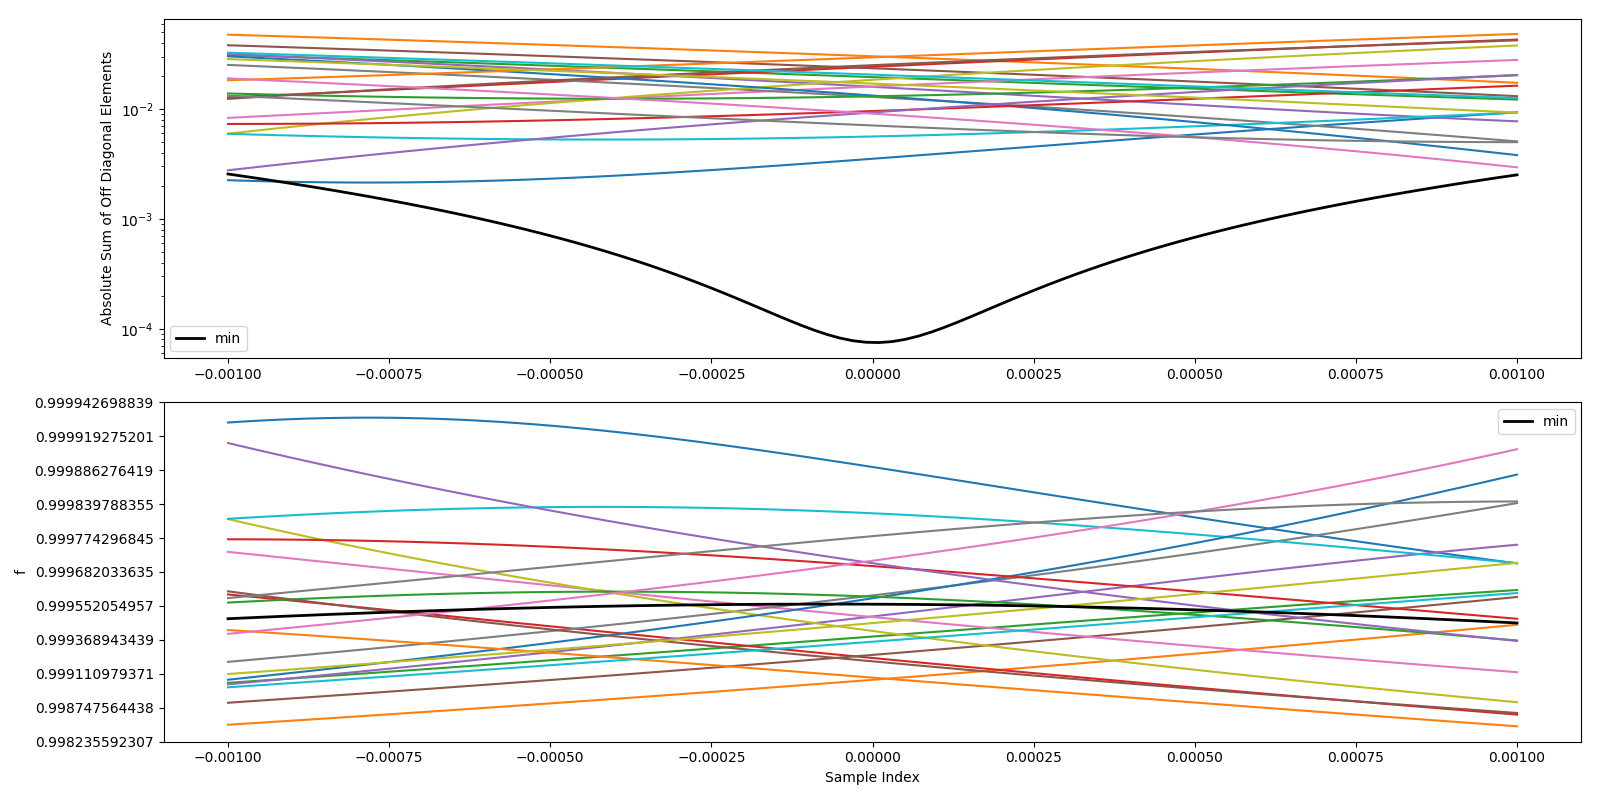
\includegraphics[width=\textwidth]{1q0.png}
% \caption{This is one example of a 1D slice varying over one control.}
% \end{subfigure}%
% ~
% \begin{subfigure}[t]{.5\linewidth}
% 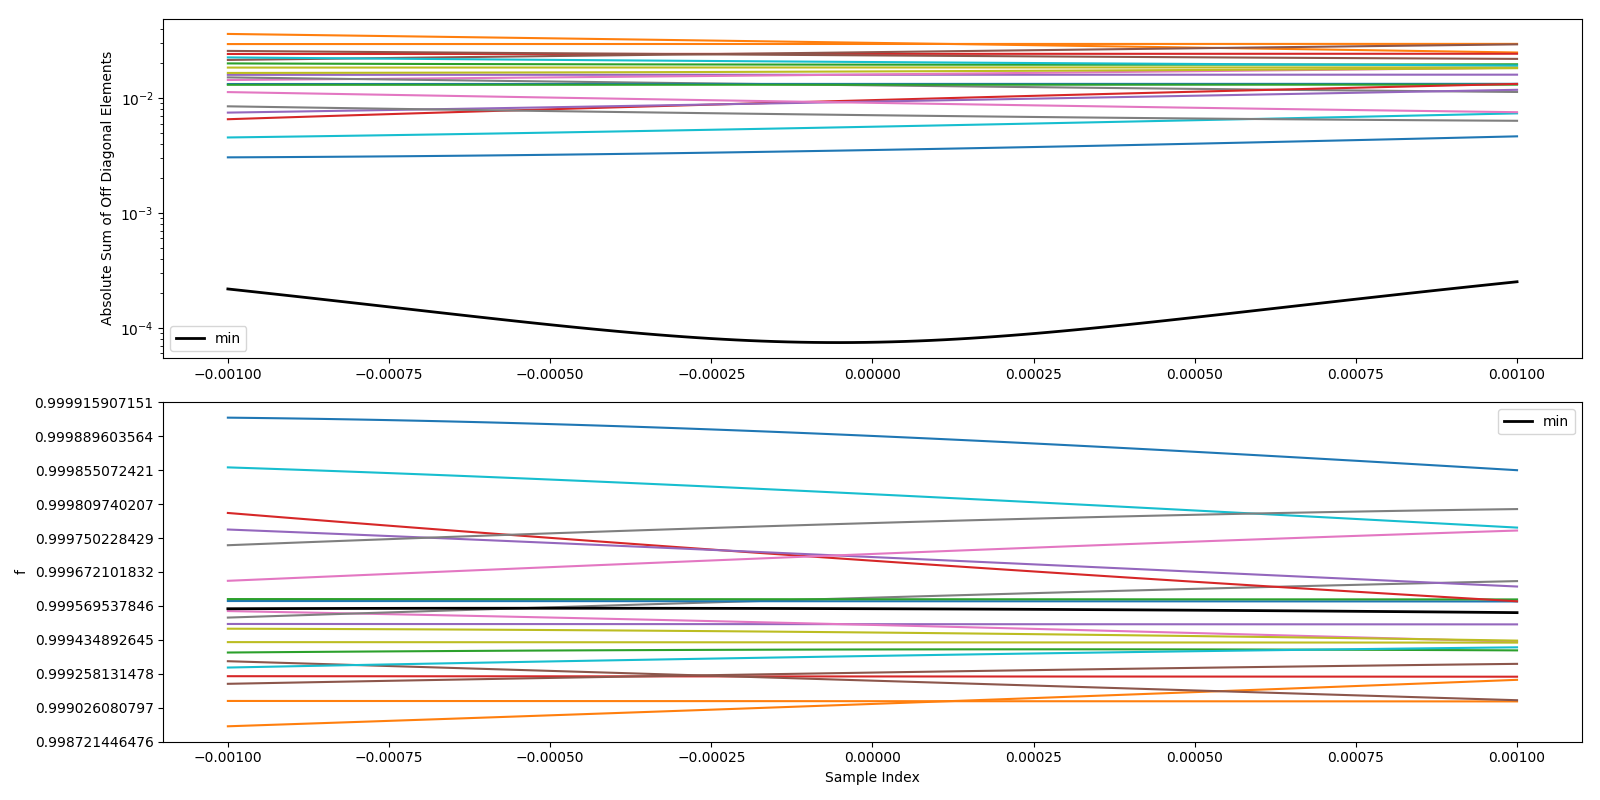
\includegraphics[width=\textwidth]{1q1.png}
% \caption{This is another example of a 1D slice varying over one control.}
% \end{subfigure}
%   \label{fig:1qnum}
% \end{figure*}



% \begin{figure*}
% \centering
% \begin{subfigure}[t]{.5\linewidth}
% 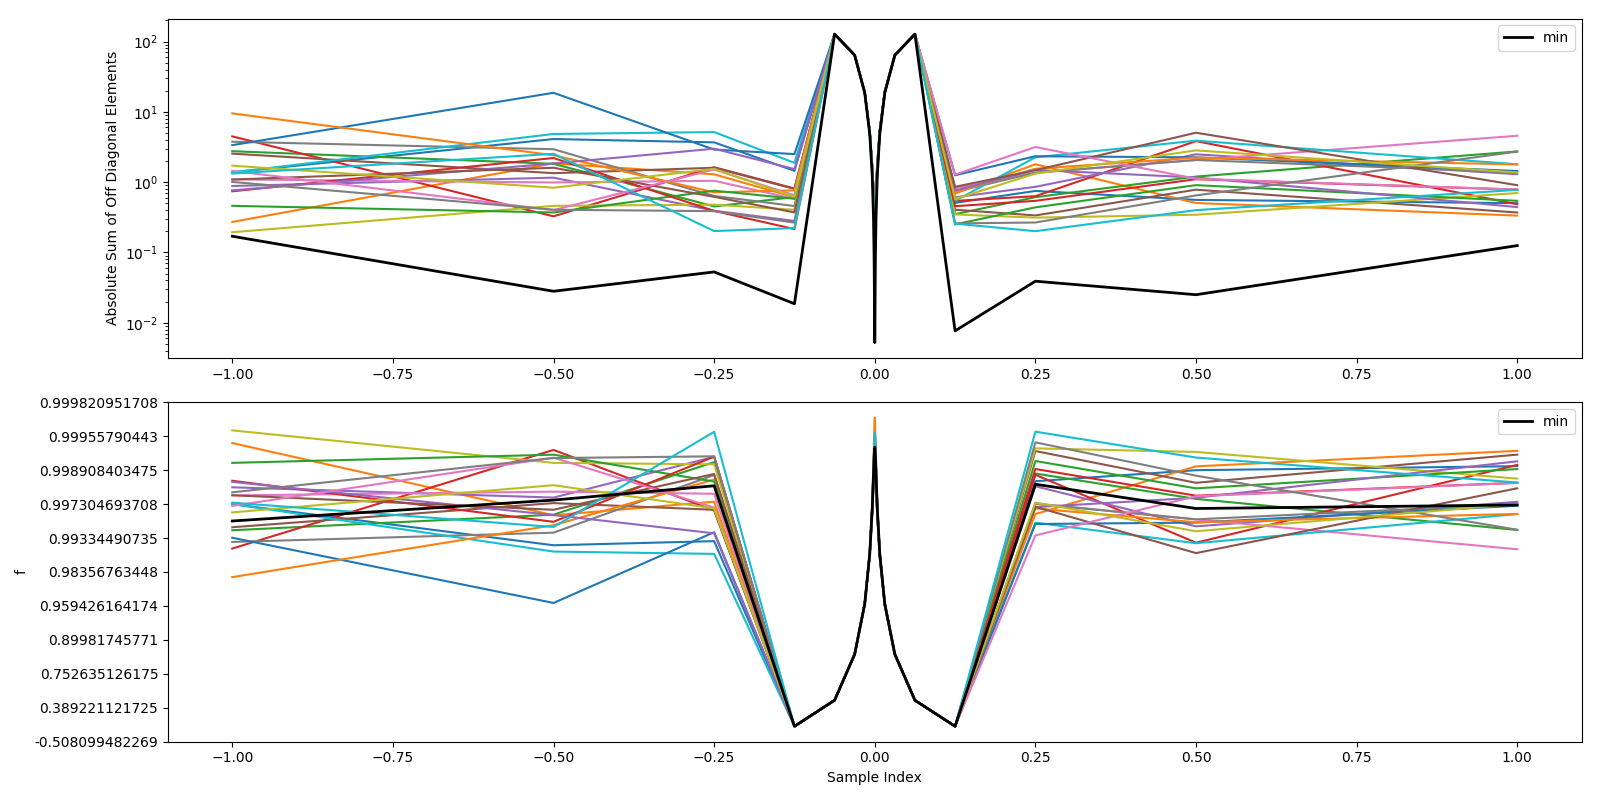
\includegraphics[width=\textwidth]{control_dpn_all0.png}
% \caption{This is one example of a 1D slice varying over one control. There are five of these in total, but only one is interesting.}
% \end{subfigure}%
% ~
% \begin{subfigure}[t]{.5\linewidth}
% 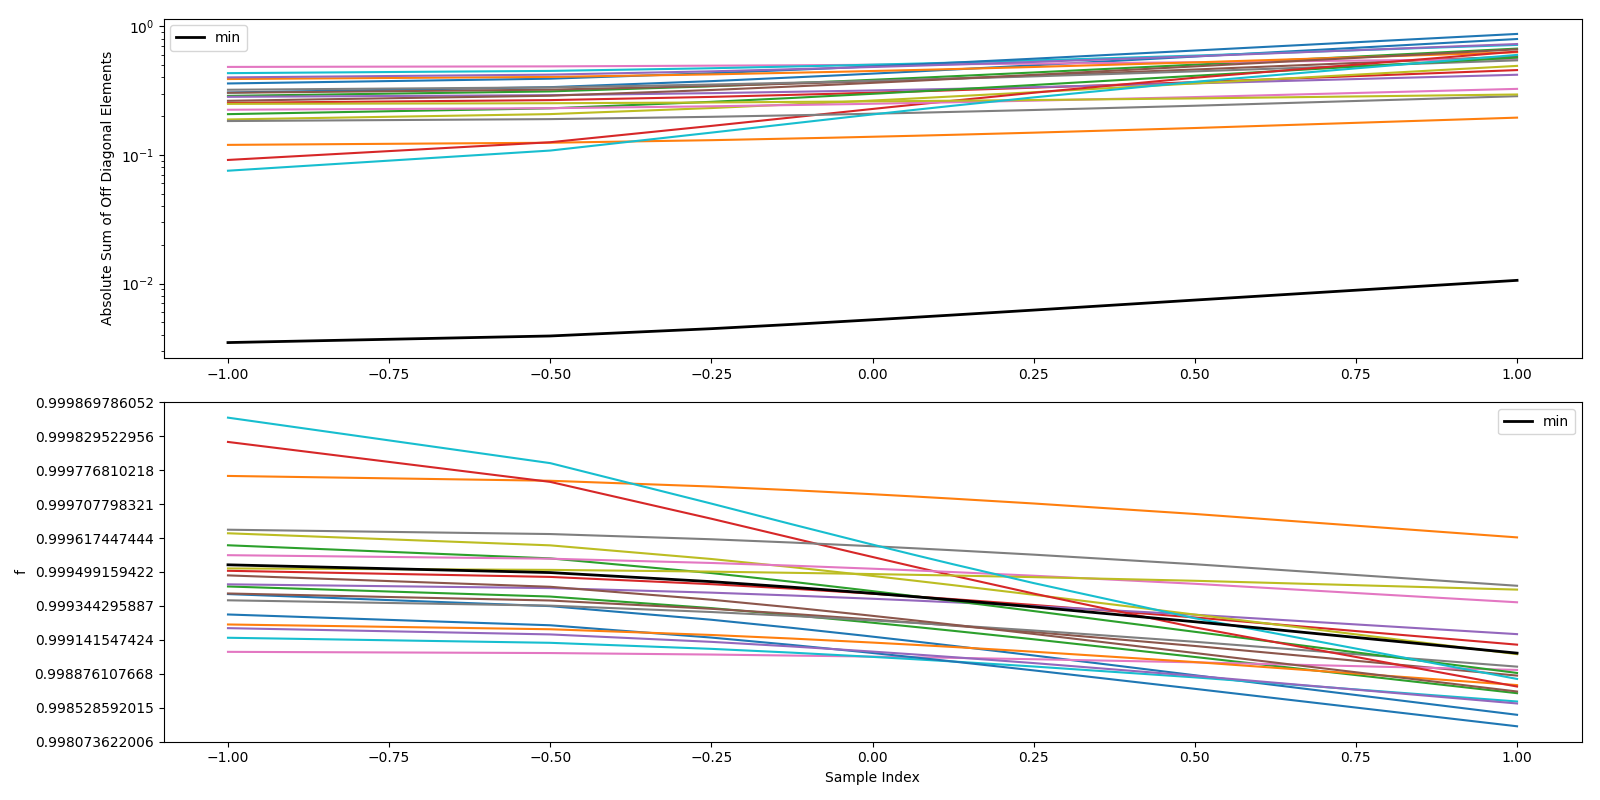
\includegraphics[width=\textwidth]{control_dpn_all2.png}
% \caption{This is one example of a 1D slice varying over one control. There are five of these in total, but only one is interesting.}
% \end{subfigure}
%   \label{fig:2qnum}
% \end{figure*}
\section{Numerical Results}\label{numerical}
\subsection{1Q Gates}\label{1Q Gates}
 In this section, we present numerical results on generating one-qubit gates that together with $RZ(\theta$) rotations are universal for one-qubit computation. Our control Hamiltonian is given as:
\begin{equation}\label{eq:1Qham}
  H = \epsilon\sigma_z + (1 + \delta)(c_x(t)\sigma_x + c_y(t)\sigma_y)
\end{equation}
where $\epsilon \sim \delta \sim \mathcal{N}(0, .001)$ We assume that the errors on $\sigma_x$ and $\sigma_y$ are perfecly correlated, as mentioned in Section \ref{ocp}. In our simulation we chose an total evolution time of $T=\pi$, and a number of steps $N=100$, with a threshold infidelity of $1E-3$.

The results can be seen in \ref{fig:1qnum}, where we have plotted each control as a function of one detuning value, fixing the others to zero. In the top half of each plot, we show the variation in the sum of the absolute valua of the off diagonal elements of the Pauli-Liouville Representation, while in the lower plot we see the variation in fidelity. While the controls were optimized by considering Gaussian noise with $\sigma=.001$ for each control, we have plotted the performance of the controls over a wider range to show more structure. We see over an order of magnitude improvement in the sum of the absolute values of the off-diagonal elements, while the fidelity remains above the specified target.



\subsection{2Q Gates}\label{2Q Gates}
 In this section, we present numerical results on a generating one and two-qubit gates that together with $RZ(\theta)$ rotations are universal for two-qubit computation. Our control Hamiltonian is given as:
\begin{equation} \label{eq:2Qham}
\begin{split}
H = &\sum_{j=1}^2(\epsilon_j\sigma_z^j + (1 + \delta_j)(c_x^jx(t)\sigma_x^j + c_y^j(t)\sigma_y^j)) \\
&+ \exp{(-i\frac{\sigma_z^1\otimes\sigma_z^2}{4})}
\end{split}
\end{equation}
We again assume that the standard deviations are $.001$ on all parameters $\delta_j$ and $c^j_i$ and that errors on the single qubit $\sigma_x$ and $\sigma_y$ rotations are perfectly correlated. In this simulation we again had a threshold infidelity of $1E-3$, but we increased the total evolution time to $T=4\pi$, and increased the number of steps to $N=400$ so that the size of each time step was the same as in the one qubit example, however the total evolution time was greater to allow GRAPE more opportunities to find non-trivial pulseshapes.

As in \ref{1qnum}, the results of these numerics can be visualized in \ref{fig2num}. Notably, even in the two qubit case where optimization over many controls becomes more difficult, we see a decrease in the magnitude of the off-diagonal terms by over an order of magnitude.


\section{Experimental Results}\label{experimental}
To demonstrate the realizability of this routine, we implemented it on a superconducting qubit, to calibrate an $RX(\frac{\pi}{2})$ pulse. The qubit being used had a FILL IN $\mu$s T1, and a FILL IN $\mu$s T2.

In this example we intentionally over and under-calibrated four pulseshapes. For each of these pulseshapes, in addition to their BCS and the calibrated pulse, we then ran a randomized benchmarking experiment.\cite{Magesan2011} The results are plotted in \ref{fig:rb}. In each case, our Clifford sequences were decomposed into RX($\frac{\pi}{2})$) and RY($\frac{\pi}{2})$) pulses.  In the superconducting qubit architecture used, these gates are implemented using the same pulse envelope definition. It was shown in \cite{Ball2016} that for a particular error model, non-Markovian, or \textit{quasi-static}, noise can result in more general Gamma Distributed noise, while Markovian noise, such as depolarizing noise, should result in Gaussian distributed fidelity estimates for each randomized benchmarking sequence depth. Our results are consistent with this, as demonstrated by the long tails in the four leftmost plots that vanish in the bottom right plot.

\begin{figure}[H]
  \centering
  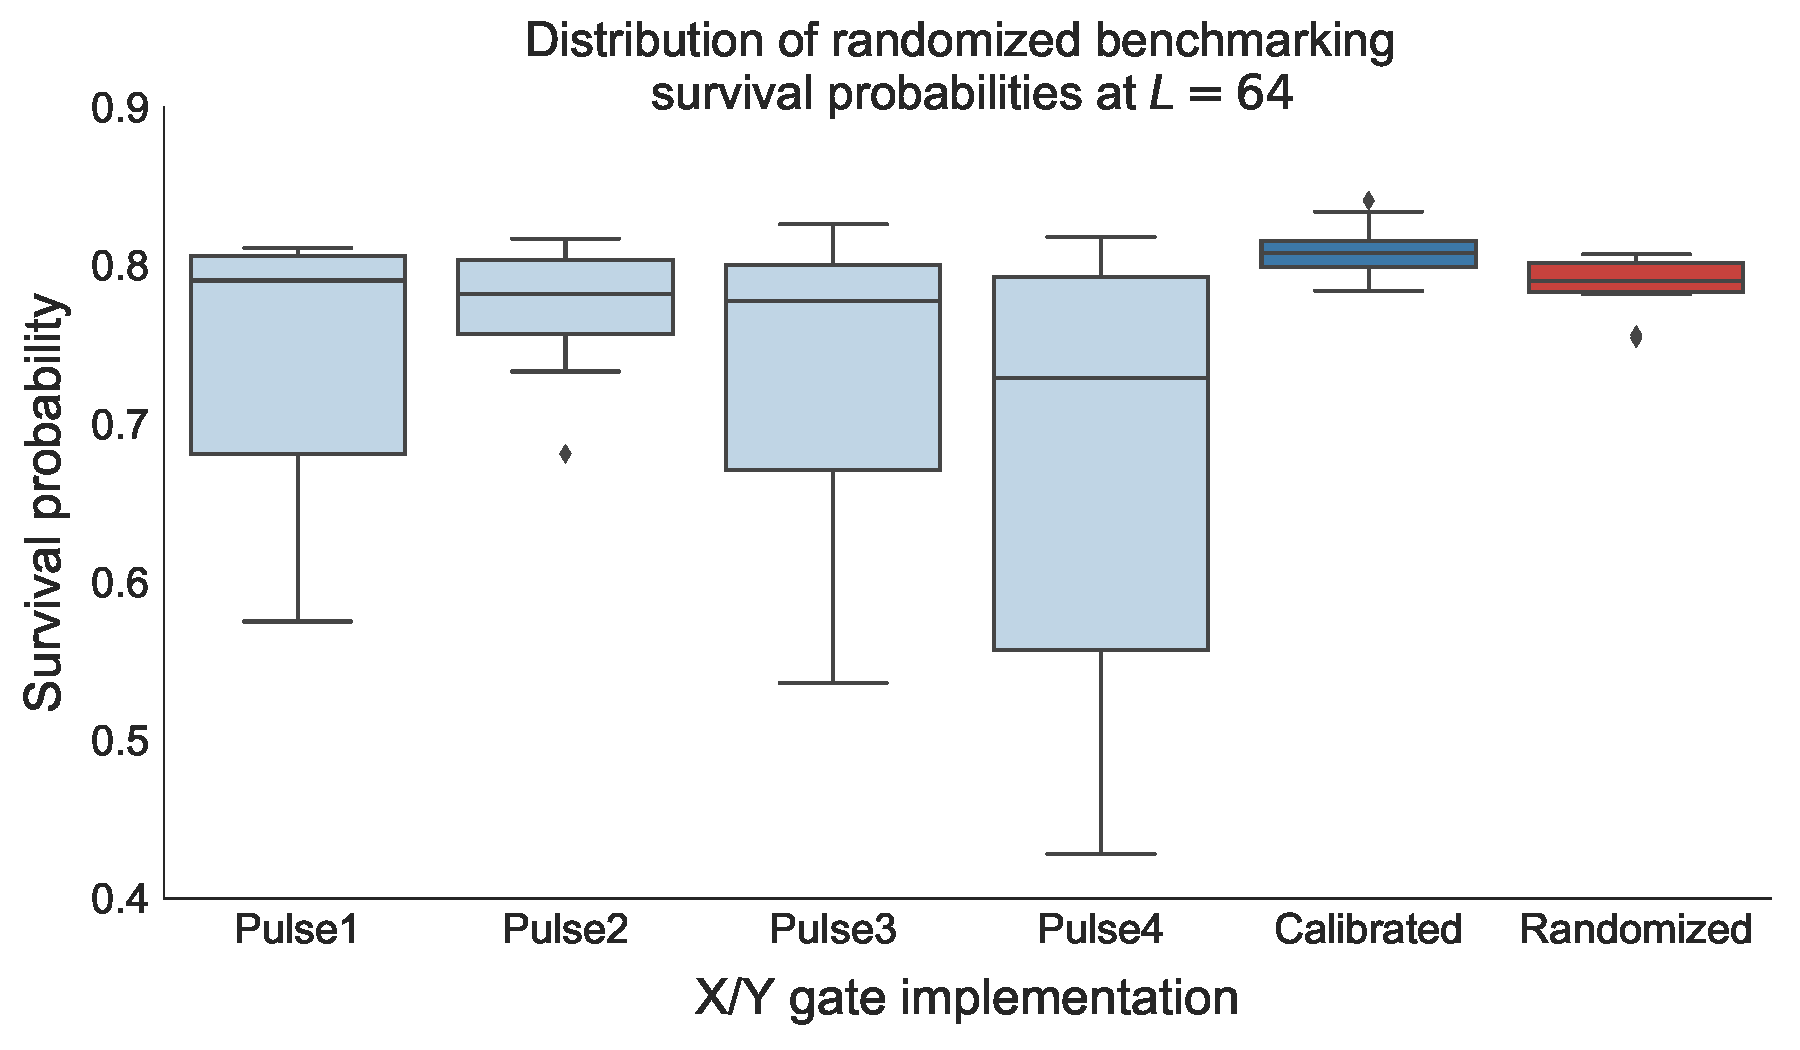
\includegraphics[width=\columnwidth]{rb_data.pdf}
  \caption{Randomized benchmarking experiments ran using different pulse definitions. The four plots on the left are from the incorrectly calibrated pulse, while the top right is the calibrated pulse, and the bottom right is the BCS.}
  \label{fig:rb}
\end{figure}

\section{Conclusion and Future Work}
We have shown numerically and experimentally that drawing from a collection of implementations of a gate with the correct probabilties can reduce coherent error by an order of magnitude, while increasing incoherent error by a smaller amount, at virtually no cost to gate fidelity. We have demonstrated that these approximate controls can be generated through optimal control, and that the minimization problem is tractable. In addition, we have shown that it is possible to perform the routine on existing hardware. The code used to generate the numerical results in this paper is available at \cite{decorrelating_errors}.

Future directions for this work include moving the random gate selection from a precompilation step to a runtime logic, investigating other optimzation routines such as CRAB \cite{Caneva2011} and GOAT\cite{Machnes2018}, and using more precise benchmarking routines such as GST\cite{BlumeKohout2017} to more quantitatively investigate the performance of these routines.

In addition, the numerical work in the paper assumed access to a model of the system. In general, an experimenter may not have a model readily available to describe the system, maybe due to on-chip crosstalk, or even if they do have access to such a model, it might be computationally intractable to simulate. In both of these situations, numerical generation of candidate pulseshapes and the minimization become infeasible. One approach would to use \textit{in situ} optimal control techniques \cite{Wu2018, Kelly2014, Ferrie2015} to generate candidate controls, and then use an optimizer like Nealder-Mead to minimize the magnitude of off-diagonal terms as measured by simple pulse sequences that amplify those elements of the process matrix.\needcite

\section{Acknowledgements}
Sandia National Laboratories is a multimission laboratory managed and operated by National Technology and Engineering Solutions of Sandia, LLC, a wholly owned subsidiary of Honeywell International, Inc., for the U.S. Department of Energy's National Nuclear Security Administration under contract DE-NA0003525.
\bibliography{decorrelation.bib}
\end{document}
